%% Submissions for peer-review must enable line-numbering 
%% using the lineno option in the \documentclass command.
%%
%% Preprints and camera-ready submissions do not need 
%% line numbers, and should have this option removed.
%%
%% Please note that the line numbering option requires
%% version 1.1 or newer of the wlpeerj.cls file, and
%% the corresponding author info requires v1.2

\documentclass[fleqn,10pt,lineno]{wlpeerj} % for journal submissions
% \documentclass[fleqn,10pt]{wlpeerj} % for preprint submissions

\title{Invasive lionfish present region-wide variation of allometric growth in
the Western Atlantic}

\author[1]{Juan Carlos Villaseñor-Derbez}
\author[1]{Sean Fitzgerald}
\affil[1]{Bren School of Environmental Sciences and Management, University of California
  Santa Barbara, Santa Barbara, California, USA}
\corrauthor[1]{Juan Carlos Villaseñor-Derbez}{jvillasenor@ucsb.edu}

% \keywords{Keyword1, Keyword2, Keyword3}

\begin{abstract}
Lionfish (\emph{Pterois volitans / miles}) are an invasive species in
the Western Atlantic and the Caribbean. Improving management of invasive
lionfish populations requires accurate estimates of total biomass, which
depend on accurate estimates of the length-weight relationship. Lionfish
exhibit a sedentary behavior that is likely to result in high levels of
spatial variation in some life history characterstics, such as the
length-weight relationship. We review 12 published length-weight
relationships of lionfish taken throughout their invasive range and
describe the spatial variation and implications of these differences.
The spatial pattern observed here is consistent with those reported in
genetic studies or age-at-length studies. We show that the use of
\emph{ex situ} parameters can result in up to a three-fold
overestimation of Total Weight, but that using parameters obtained
nearby reduces this error. These findings can have major implications
for management in terms of predicting effects on local ecosystems,
evaluating the effectiveness of removal programs, or estimating biomass
available for harvest.
\end{abstract}

\begin{document}

\flushbottom
\maketitle
\thispagestyle{empty}

\section*{Introduction}

Lionfish (\emph{Pterois volitans/miles} complex) are an invasive species
in the western Atlantic and Caribbean Sea, likely introduced through
liberation of aquarium-kept organisms \citep{betancurr_2011}. They are
the first invasive marine vertebrates established along the North
Atlantic Caribbean coasts
\citep{schofield_2009,schofield_2010,sabidoitza_2016} and their presence
has been labeled as a major marine invasion because they threaten local
biodiversity, spread rapidly, and are difficult to manage
\citep{hixon_2016}.

Invasive lionfish are primarily studied in coral reef ecosystems, where
their impacts are far-reaching. For example, field experiments by
\citet{albins_2008} showed that lionfish establishment led to reduced
recruitment of native fishes by nearly 80\% over a five week period in
Florida. \citet{green_2012} report that prey fish biomass declined 65\%
over two years as lionfish biomass increased along Bahamian coral reefs.
Lionfish have also established invasive populations in other habitats
such as estuaries, mangroves, hard-bottomed areas, and mesophotic reefs
\citep{jud_2011,barbour_2010,muoz_2011,andradibrown_2017,claydon_2012}.

A substantial amount of research describes lionfish feeding ecology
throughout the invaded range
\citep{muoz_2011,morris_2009,cote_2013,dahl_2014,valdezmoreno_2012,villaseorderbez_2014,hackerott_2017,sandel_2015}.
A meta-analysis by \citet{peake_2018} showed that invasive lionfish prey
on at least 167 different species across the tropical and temperate
North Atlantic. Their feeding behavior and high consumption rates can
reduce recruitment and population sizes of native reef-fish species, and
can further endanger reef fish
\citep{albins_2008, green_2012,rocha_2015}. (However, see
\citet{hackerott_2017} for a case where there was no evidence that
lionfish affected the density, richness, or community composition of
prey fishes). Major efforts have been made to understand the possible
impacts of the invasion by tracking the spread of established lionfish
populations through time \citep{schofield_2009,schofield_2010} and by
predicting invasion ranges under future climates \citep{grieve_2016}.
It\{s been proposed that trophic impacts of lionfish can be minimized if
local lionfish biomass is controled by culling
\citep{ariasgonzalez_2011}.

Governments and non-profit organizations have sought to reduce lionfish
densities through removal programs and incentivizing its consumption
\citep{chin_2016}. In some cases, these have shown to significantly
reduce --but not quite eliminate-- lionfish abundances at local scales
\citep{sandel_2015,chin_2016,deleon_2013}. In addition, culling programs
can help stabilize or grow native prey fish populations
\citep{cote_2014}. Complete eradication of lionfish through fishing is
unlikely because of their rapid recovery rates and ongoing recruitment
to shallow-water areas from their persistent populations in mesophotic
coral ecosystems \citep{barbour_2011,andradibrown_2017}. However,
promoting lionfish consumption might create a level of demand capable of
sustaining a stable fishery, which can help control shallow-water
populations while providing alternative livelihoods and avoiding further
impacts to local reef biota \citep{chin_2016}.

The feasibility of establishing fisheries through lionfish removal
programs has been extensively evaluated through field observations and
empirical modeling
\citep{barbour_2011,morris_2011,deleon_2013,johnston_2015,sandel_2015,chin_2016,usseglio_2017}.
One contributing factor to the success of many removal programs is the
sedentary nature of adult lionfish \citep{jud_2012}. Culling programs
are effective in reducing local adult populations largely because
lionfish exhibit high levels of site fidelity and rarely leave their
home range \citep{Fishelson_1997,cote_2014,kochzius_2005}. Fish with
this sedentary behavior are likely to exhibit high levels of spatial
variation in important life history characterstics such as growth or
natural mortality rates \citep{hutchinson_2008,wilson_2012}. The
importance of considering spatial heterogeneity is well-documented in
terms of assessing and managing sedentary species
\citep{gunderson_2008,guan_2013}, and such variation should be accounted
for when evaluating the feasibility of establishing lionfish fisheries
as well.

Determining the feasibility of such initiatives require modeling changes
in biomass in response to changes in mortality (\emph{i.e.} culling). A
common way to model this is via length-structured population models,
where fish lengths are converted to weight to calculate total biomass
\citep{cote_2014,barbour_2011,andradibrown_2017}. The length-weight
relationship is therefore an essential component of these models, but
this relationship can vary across regions as a response to biotic
(\emph{e.g.} local food availability) and abiotic (\emph{e.g.} water
temperature) conditions \citep{johnson_2016}. Literature suggests that
site-specific parameters are necessary in order to accurately estimate
biomass when length-weight relationships are spatially variable, and
this variability becomes increasingly important when estimating the
potential effectiveness and feasability of lionfish culling programs or
when identifying total biomass available for harvest by fishers
\citep{barbour_2011,morris_2011,johnston_2015,chin_2016,cote_2014}. In
addition to environmentally-driven spatial variation, genetic analysis
of invasive lionfish suggest biological differences due to the existence
of two genetically distinct subpopulations between the northwest
Atlantic and the Caribbean \citep{betancurr_2011}. To date, no studies
have examined region-wide differences in length-weight parameters
despite the large number of studies reporting this relationship for
lionfish.

The objective of this paper is to describe the spatial pattern of
length-weight relationships of lionfish in the Caribbean and Western
Atlantic and evaluate the implications of these spatial differences.
Length-weight relationships for lionfish exist for North Carolina,
Northern and Southern Gulf of Mexico, the Southern Mexican Caribbean,
Bahamas, Little Cayman, Jamaica, Bonaire, Puerto Rico, and Costa Rica
\citep{barbour_2011,fogg_2013,dahl_2014,aguilarperera_2016,sabidoitza_2016,sabidoitz_2016,darling_2011,edwards_2014,chin_2016,deleon_2013,toledohernndez_2014,sandel_2015}.
This study also provides the first length-weight relationship for the
central Mexican Caribbean.

\clearpage

\section*{Materials and Methods}

We reviewed 12 published studies and obtained 17 length-weight
relationships for the North Atlantic (n = 1), Gulf of Mexico (n = 7),
and Caribbean (n = 10, Table \ref{tab:all_params}, Fig
\ref{fig:all_allo}). We collected information on sampling methods, sex
differentiation, location, and depth ranges from each study when
available, and assumed both genders were included in a study if gender
was unspecified. Only two studies reported parameters for each gender
\citep{aguilarperera_2016,fogg_2013}. Reviewed studies presented
information for organisms obtained at depths between 0.5 m and 57 m.
Three studies explicitly stated that their organisms were sampled with
pole spears
\citep{aguilarperera_2016,chin_2016,dahl_2014,sabidoitz_2016}, and five
studies mentioned that some of their organisms were obtained with pole
spears (or other type of harpoon) but also hand-held nets or fish traps
\citep{sandel_2015,barbour_2011,fogg_2013,edwards_2014,sabidoitza_2016,sabidoitz_2016,toledohernndez_2014},
and two studies did not specify how organisms were sampled
\citep{deleon_2013,darling_2011}. \citet{fogg_2013} use spine-less
weight in the length-weight relationship estimation, and thus their
parameters likely underestimate total wieght. Since no spine-less to
total weight conversions were available, these parameters were taken as
reported.

We also collected data from 10 sampling sites along the central Mexican
Caribbean coast in 2010 (Table S1). Sampling locations included wall and
carpet reefs at depths between 5.7 m and 38.1 m. All observed lionfish
(n = 109) were collected using hand nets and numbered collection
bottles. The use of hand nets prevented any weight loss due to bleeding
and allowed better representation of small sizes by eliminating gear
selectivity. Organisms were euthanized via pithing and Total Length (TL;
mm) and Total Weight (TW; g) were recorded.

\begin{figure}
\centering
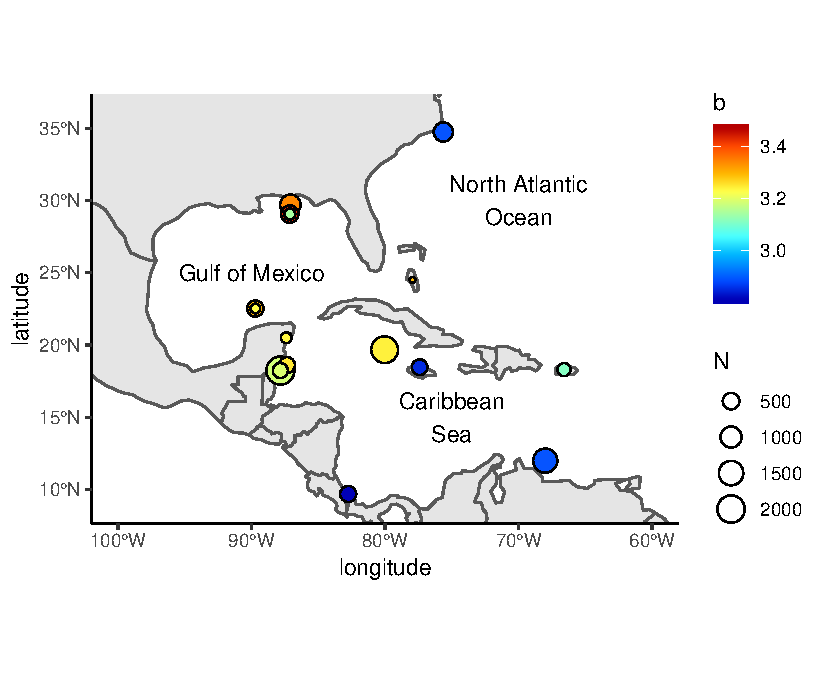
\includegraphics{Manuscript_files/figure-latex/unnamed-chunk-1-1.pdf}
\caption{\label{fig:map}Locations where allometric growth parameters of
lionfish (\emph{Pterois spp}) have been reported. Circle sizes indicate
sample size from each study, colors indicate the \(b\) coefficient from
Eq. \ref{eq:allometric}.}
\end{figure}

The weight at length relationship for lionfish in the central Mexican
Caribbean was calculated with the allometric growth function:

\begin{equation}
\label{eq:allometric}
TW = aTL^b
\end{equation}

Where \(a\) is the ponderal index and \(b\) is the scaling exponent or
allometric parameter. When \(b = 3\), it is said that the organism
exhibits a perfect isometric growth. Transforming this equation via
base-10 logarithms:

\begin{equation}
\label{eq:log-alo}
log_{10}(TW) = b\times log_{10}(TL) + log_{10}(a)
\end{equation}

This can be simplified and re-written as:

\begin{equation}
\label{eq:log-alo-trans}
Y = bX + c
\end{equation}

Where \(Y = log_{10}(TW)\), \(X = log_{10}(TL)\), and
\(c = log_{10}(a)\). The coefficients (\(c\) and \(b\)) were estimated
with an Ordinary Least Squares Regression and heteroskedastic-robust
standard error correction \citep{zeileis_2004}. The \(b\) coefficient
was tested against the null hypothesis of isometric growth (\emph{i.e.}
\(H_0: b = 3\)). Coefficients were tested with a two-tailed Student's t,
and the significance of the regression was corroborated with an F-test.

Some of the reviewed studies inconsistently defined \(a\) as either the
ponderal index from Eq. \ref{eq:allometric} or the y-intercept (\(c\))
from Eq. \ref{eq:log-alo-trans}. Other studies incorrectly reported
parameters as mm-to-g conversions when they were in fact cm-to-g
conversions. We standardized each study by converting coefficients and
report all parameters as TL(mm) to TW (gr) conversions. Locations where
allometric studies have been performed are shown in Figure \ref{fig:map}
and Table \ref{tab:all_params}.

Combining the length-weight parameters extracted from the literature and
the additional pair calculated here, we obtain a total of 18 pairs. We
use the central Mexican Caribbean as a case study of how the use of
\emph{ex situ} parameters influences the accuracy of weight estimates
for lionfish. We estimated TW from the TL observations we collected in
the central Mexican Caribbean (n = 109) using each of the 18 parameter
pairs and divided predicted weights by known observed weights to obtain
a simple measure of over- or underestimation. Difference in mean weight
ratios across the different parameter pairs were tested with a one-way
analysis of variance (ANOVA) and Tuskey's test was used for post-hoc
tests. All analyses were performed in R version 3.5.0
\citep{rcore_2018}. Raw data and code used in this work are available at
dryad.org.

\section*{Results}

The length-weight relationship for organisms from the central Mexican
Caribbean resulted in the coefficient values
\(a = 3.2056297\times 10^{-6}\), \(b = 3.2347391\) and
\(c = -5.4940866\) (\(R^2 = 0.977\), F(df = 1; 107) = 6928.67,
\(p < 0.001\)). The allometric factor (\(b\)) was significantly
different from \(b = 3\) (\(t(107) = 6.04; p<0.001\)) indicating that
lionfish present allometric growth. The length-weight coefficients
estimated in this study were within the range identified by studies in
other regions (Table \ref{tab:all_params}). Figure \ref{fig:l-w-carib}
shows the relationship between TL and TW for this region, and more
information on model fit is presented in Table S2.

Figure \ref{fig:all_allo} shows the length-weight relationships with
parameters from all studies. Parameters from models fit to males or
females exclusively tend to have a higher steepness (\emph{i.e.} higher
allometric parameter), with mean \(\pm\) standard deviation values of
\(b = 3.27 \pm 0.06\) and \(b = 3.31 \pm 0.23\) for males and females
respectively, compared to parameters from models for combined genders
with a mean \(\pm\) standard deviation value of \(b = 3.14 \pm 0.20\).
In the case of the ponderal index (\(a\)) and its \(log_{10}\)
transformation (\(c\)), values were higher for parameters for combined
genders.

There were significant differences in our predicted weights for the
central Mexican Caribbean when using the different pairs of parameters
(\(F(df = 15; 1728) = 38.26; p < 0.001\)). Weight estimates using
parameters from the Gulf of Mexico and North-Western Atlantic were
higher on average than those from the Caribbean. The average (\(\pm\)
SD) predicted-to-observed weight ratios from these three regions were
1.24 \(\pm\) 0.309, 1.76 \(\pm\) 0.496, and 1.17 \(\pm\) 0.398,
respectively. The lowest weight estimates resulted from using the
allometric parameters from Banco Chinchorro in the Caribbean
\citet{sabidoitz_2016}, and the highest weight estimates came from the
Northern Atlantic \citep{barbour_2011}. The calculated ratio of
predicted-to-observed weight ranged from 0.80 \(\pm\) 0.19 to 1.76
\(\pm\) 0.50 (mean \(\pm\) SD). Tukey's post-hoc test suggests that
weight ratios for the central Mexican Caribbean were not differnt from
those obntained with parameters from Little Cayman, the Bahamas, and
some sites in the Gulf of Mexico (Tukeys HSD \(p > 0.05\)).
Predicted-to-observed weight ratios are presented in Figure
\ref{fig:bio_ratio}. Spine-less weight parameters from \citet{fogg_2013}
still produced predicted-to-observed weight ratios \textgreater{} 1.

\begin{figure}
\centering
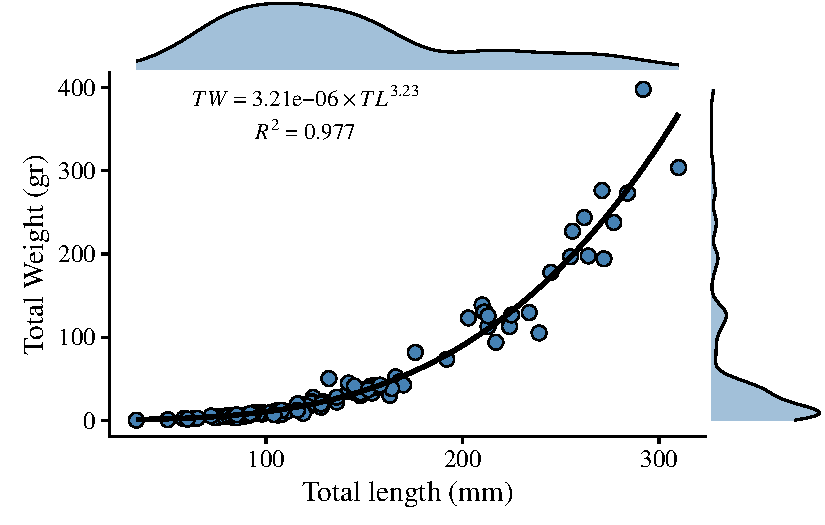
\includegraphics{Manuscript_files/figure-latex/unnamed-chunk-4-1.pdf}
\caption{\label{fig:l-w-carib}Length-weight relationship for 109
lionfish sampled in the central Mexican Caribbean. Points indicate
samples, dashed black line indicates curve of best fit, marginal plots
represent the density distribution of each variable.}
\end{figure}

\begin{table}

\caption{\label{tab:unnamed-chunk-5}\label{tab:all_params}Summary of 18 allometric growth parameters available for lionfish in the invaded range from peer-reviewed literature and this study. All parameters have been adjusted to convert from millimeters to grams. n = Sample size, Sex specifies whether data was presented for Females (F), Males (M), or both genders combined (B), a = scaling parameter for Eq. 1 (presented in $\times 10^{-5}$), c = y-intercept for Eq. 3, b = exponent or slope for Eq. 1 or Eq. 3, respectively. The $R^2$ column indicates reported model fit.}
\centering
\begin{tabular}[t]{llllrrll}
\toprule
Region & Sex & n & a & b & c & \$R\textasciicircum{}2\$ & Reference\\
\midrule
Caribbean & B & 458 & 3.6 & 2.81 & -4.44 & - & Sandel et al., 2015\\
Caribbean & B & 419 & 2.8 & 2.85 & -4.56 & 0.8715 & Chin et al., 2016\\
Caribbean & B & 1450 & 2.3 & 2.89 & -4.64 & 0.96 & de Leon et al., 2013\\
Caribbean & B & 1887 & 0.3 & 3.24 & -5.52 & 0.97 & Edwards et al., 2014\\
Caribbean & B & - & 0.25 & 3.29 & -5.60 & - & Darling et al., 2011\\
\addlinespace
Caribbean & B & 2143 & 0.52 & 3.18 & -5.28 & 0.9907 & Sabido-Itza et al., 2016\\
Caribbean & B & 227 & 0.8 & 3.11 & -5.10 & 0.958 & Toledo-Hernández et al., 2014\\
Caribbean & B & 449 & 0.23 & 3.25 & -5.64 & 0.97 & Sabido-Itza et al., 2016b\\
Caribbean & B & 368 & 0.32 & 3.19 & -5.50 & 0.98 & Sabido-Itza et al., 2016b\\
Caribbean & B & 109 & 0.32 & 3.23 & -5.49 & 0.9766 & This study\\
\addlinespace
GoM & B & 934 & 0.21 & 3.34 & -5.68 & 0.98 & Dahl \& Patterson, 2014\\
GoM & B & 472 & 0.29 & 3.30 & -5.54 & 0.95 & Aguilar-Perera \& Quijano-Puerto, 2016\\
GoM & F & 67 & 0.12 & 3.47 & -5.93 & 0.95 & Aguilar-Perera \& Quijano-Puerto, 2016\\
GoM & M & 59 & 0.42 & 3.23 & -5.38 & 0.95 & Aguilar-Perera \& Quijano-Puerto, 2016\\
GoM & B & 582 & 0.14 & 3.43 & -5.86 & 0.99 & Fogg et al., 2013\\
\addlinespace
GoM & M & 119 & 0.27 & 3.31 & -5.57 & 0.97 & Fogg et al., 2013\\
GoM & F & 115 & 0.68 & 3.14 & -5.17 & 0.94 & Fogg et al., 2013\\
North Atlantic & B & 774 & 2.9 & 2.89 & -4.54 & - & Barbour et al.,2011\\
\bottomrule
\end{tabular}
\end{table}

\begin{figure}
\centering
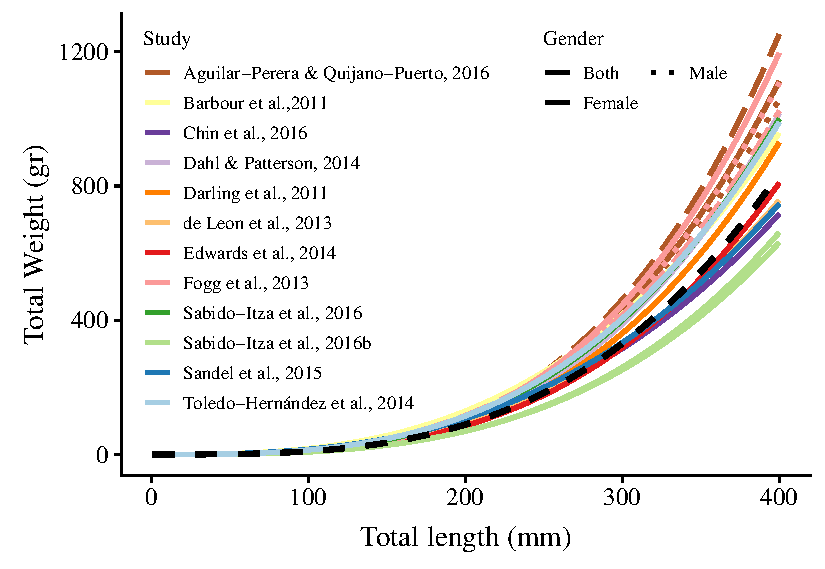
\includegraphics{Manuscript_files/figure-latex/unnamed-chunk-6-1.pdf}
\caption{\label{fig:all_allo}Length-weight relationships (n = 18) for 12
studies and this study. Colors indicate studies from which the
parameters were extracted. Dotted, dashed and solid lines show models
for males, females, and combined sexes, respectively. The dashed black
line represents the relationship estimated in this study.}
\end{figure}

\begin{figure}
\centering
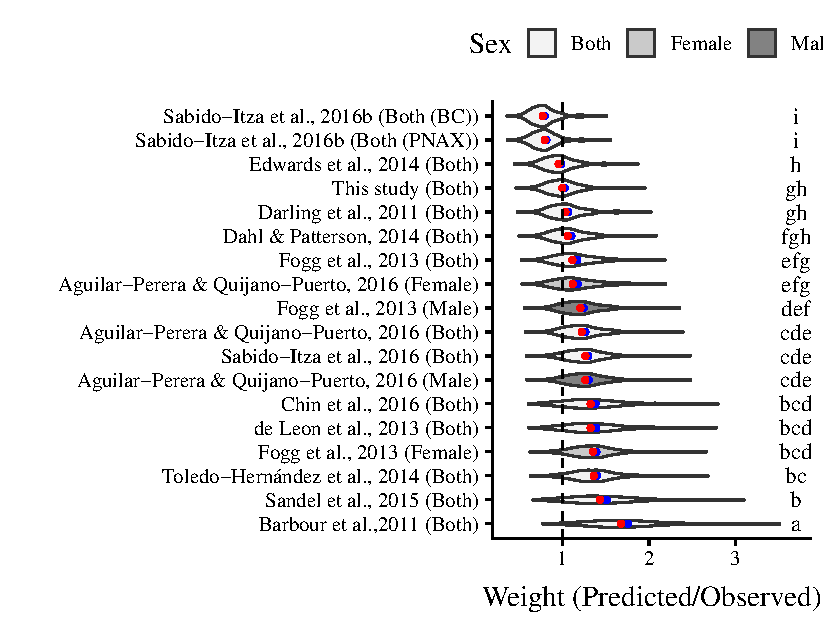
\includegraphics{Manuscript_files/figure-latex/unnamed-chunk-7-1.pdf}
\caption{\label{fig:bio_ratio}Violin plot of predicted-to-observed
weight ratios for 18 pairs of allometric parameters. Red and blue
circles indicate median and mean values, respectively. Like letters
indicate values that do not differ significantly.}
\end{figure}

\clearpage

\section*{Discussion}

We detected substantial differences in weight-at-length between
organisms from the Caribbean and Gulf of Mexico / North-Western
Atlantic. The groupings of predicted-to-observed weight ratios were
consistent with the spatial distribution of the studies, suggesting that
these differences are mediated by space. These length-weight differences
mirror similar findings of regional variability in age-at-length
relationships of lionfish across both their invaded and native regions
\citep{pusack_2016}. These patterns may be driven by genetic variation
or by organisms being exposed to distinct environmental conditions. For
example, \citet{betancurr_2011} used mitochondrial DNA to demonstrate
the existence of two distinct population groups, identified as the
``Caribbean group'' and ``Northern Group'', and \citet{fogg_2015}
alternatively suggested that age-at-length differences may be driven by
climate. Differences in weight-at-length could also reflect differences
in energy input or differential usage of this energy, or a combination
of both. Future research is needed to determine which processes are at
work here.

Differences in length-weight relationships have traditionally been
highlighted as potential pitfalls to fishery management. For example,
\citet{wilson_2012} show that small-scale variations in length-at-age
and fishing mortality in other Scorpaeniformes translate to differential
landings, effort, and catch per unit effort in the live fish fishery of
California, and that these differences must be taken into account in
management plans. The lionfish case poses the opposite scenario, where
the manager desires to erradicate species. To accurately gauge both the
effectiveness of lionfish removal efforts and the resources needed to
successfully manage an invasion, we must acknowledge and understand
regional biological differences in important variables such as
allometric growth parameters.

The results presented here have major implications for management. For
example, \citet{edwards_2014} simulated a lionfish culling program under
two scenarios, one using length-at-age and length-to-weight parameters
from North Carolina and one using parameters from Little Cayman. Their
results show that using different parameters caused up to a four-year
difference in the time required for the simulated lionfish population to
recover to 90\% of its initial biomass after removals ceased. Here, we
show that using one set of length-weight parameters versus another for a
given length can result in up to a threefold TW overestimation. These
spatially-driven differences become especially important when allocating
resources for lionfish removal programs, incentivizing its fishery as a
source of alternative livelihoods, or estimating ecosystem impacts.
Research efforts focused on invasive lionfish populations need to use
parameters calculated for their region to the extent possible, or at
least use reasonable sets of different parameters that provide upper and
lower bounds in their results.

\section*{Aknowledgements}

The authors would like to thank thank Nils Van Der Haar and Michael
Doodey from Dive Aventuras as well as Guillermo Lotz-Cador who provided
help to collect samples.

\bibliography{references}

\end{document}